%----------------------------------------------------------------------------------------
%	SECTION 2
%----------------------------------------------------------------------------------------

\section{Engineering Analysis (EA)} \label{EA}

\subsection*{EA1(i, b, m)} 

\begin{wraptable}{r}{0.2\textwidth}
	\begin{tabular}{|ll|}
		\hline
		\multicolumn{2}{|c|}{\cellcolor[HTML]{F8A102}\textbf{EA1(i, b, m) \nomaster}} \\ \hline
		\EPA & \DSA \\
		\TPS & \LAB \\ \hline
	\end{tabular}
\end{wraptable}

In some courses, I have conducted laboratory experiments and modelling exercises.
This has further developed my skills in monitoring, interpreting and applying the results of analysis and modelling to bring about continuous improvement [EA1i].
\textit{Laboratory Project} went a step further and taught me the principles and process to engineering a better solution [EA1b and EA1m].
These principles were applied in an engineering project which aimed to optimise the design of a cooling coil.
Having earned As on all of the courses listed in the course box shows that I have an understanding of engineering principles and the ability to apply them to analyse key engineering processes.







\newpage
\subsection*{EA2(i, -)}

\begin{wraptable}{r}{0.2\textwidth}
	\begin{tabular}{|ll|}
		\hline
		\multicolumn{2}{|c|}{\cellcolor[HTML]{F8A102}\textbf{EA2(i, -) \nomaster}} \\ \hline
		\ConTechOne & \Acoustics \\
		\HYD & \EPA \\
		\TPS & \PRJ \\
		\LAB &  \\
		Arup & Sweco \\ \hline
	\end{tabular}
\end{wraptable}

A range of courses have developed my ability to understand and explain the performance of systems and components through the use of quantitative/ analytical methods and/ or modelling techniques.
For example, in \textit{Hydraulics and Hydrology A}, I learned how to use quantitative methods to distinguish laminar flows from turbulent flows.
And when we were studying thermofluids in \textit{Laboratory Project}, I used both CFD modelling and analytical methods to understand and describe the performance of a cooling coil in an air conditioning unit.

I have also applied quantitative/ analytical methods and/ or modelling techniques to classify and describe the performance of systems during my work placements at Arup and Sweco.
In particular, at Sweco I used a combination of the aforementioned methods and techniques to describe the performance of some buildings in terms of solar heat gain, energy consumption, thermal comfort, and daylighting.
The results of these analyses were then classified according to the criteria of \textit{Miljöbyggnad}: Gold, Silver, Bronze or Disapproved (see Figure~\ref{fig:svl}).








\subsection*{EA3(i, b, m)} \label{EA3}

\begin{wraptable}{r}{0.2\textwidth}
	\begin{tabular}{|ll|}
		\hline
		\multicolumn{2}{|c|}{\cellcolor[HTML]{F8A102}\textbf{EA3(i, b, m) \nomaster}} \\ \hline
		\MechB & \HYD \\
		\DPB & \DSA \\
		\EnBldgs & \TPS \\
		\PRJ & \LAB \\ \hline
	\end{tabular}
\end{wraptable}

I have developed the ability to use the results of analysis and apply quantitative and computational methods to solve engineering problems and subsequently recommend or implement appropriate action in some courses.
For example, a combination of calculations, CFD modelling and a physical laboratory experiment were used to optimise the design of a cooling coil in \textit{Laboratory Project}.
This was an iterative process of solving problems and implementing appropriate actions to come up with a better solution, for which I earned an A.
However, I do not think I have ever used alternative approaches to solve engineering problems and implement appropriate action [EA3m]; this is a skill I need to develop.







\subsection*{EA4(i, b, m)}

\begin{wraptable}{r}{0.2\textwidth}
	\begin{tabular}{|ll|}
		\hline
		\multicolumn{2}{|c|}{\cellcolor[HTML]{F8A102}\textbf{EA4(i, b, m) \nomaster}} \\ \hline
		\CAS & \EnBldgs \\
		\PRJ & \WSD \\ \hline
	\end{tabular}
\end{wraptable}

Some courses have contributed to my understanding of, and ability to apply, an integrated or systems approach to solving complex engineering problems through know-how of the relevant technologies and their application.
I would not say this skill is fully developed though as I have not had many opportunities to develop it.
An example of when I did fully demonstrate my ability to achieve LOs EA4i, EA4b and EA4m is my natural lighting design of Newington Library in \CASTitle.
With the aim of maximising daylight and avoiding direct sunlight, I had to take several aspects into consideration in the fenestration design:
\begin{itemize}
	\item The building orientation and sun path
	\item The characteristics and desirability of the natural light hitting each fa{\c{c}}ade
	\item Functions of the internal and external spaces and their required lighting levels
	\item Type of glazing (double/ triple, clear/ frosted)
	\item Subsequent thermal comfort and energy loads related to the choice of glazing
\end{itemize}


I will give an example to demonstrate the interdependent nature of this design exercise.
The south-west corner of the library housed a shelving and study area.
However, the south-west fa{\c{c}}ade would be receiving an intense afternoon sunlight, which was undesirable due to glare and the sunlight's detrimental effects on the books.
I therefore designed clerestory glazing to (a) limit direct incoming sunlight, (b) exclude distracting, unattractive or intrusive views, and (c) allow shelving against wall (see Figure~\ref{fig:nl}).
Additionally, the clerestory glazing was frosted to disperse the sunlight's rays.
My natural lighting design was commended by the judges of the course's design competition (see Figure~\ref{fig_award}).


\begin{figure}[htbp]
	\centering
	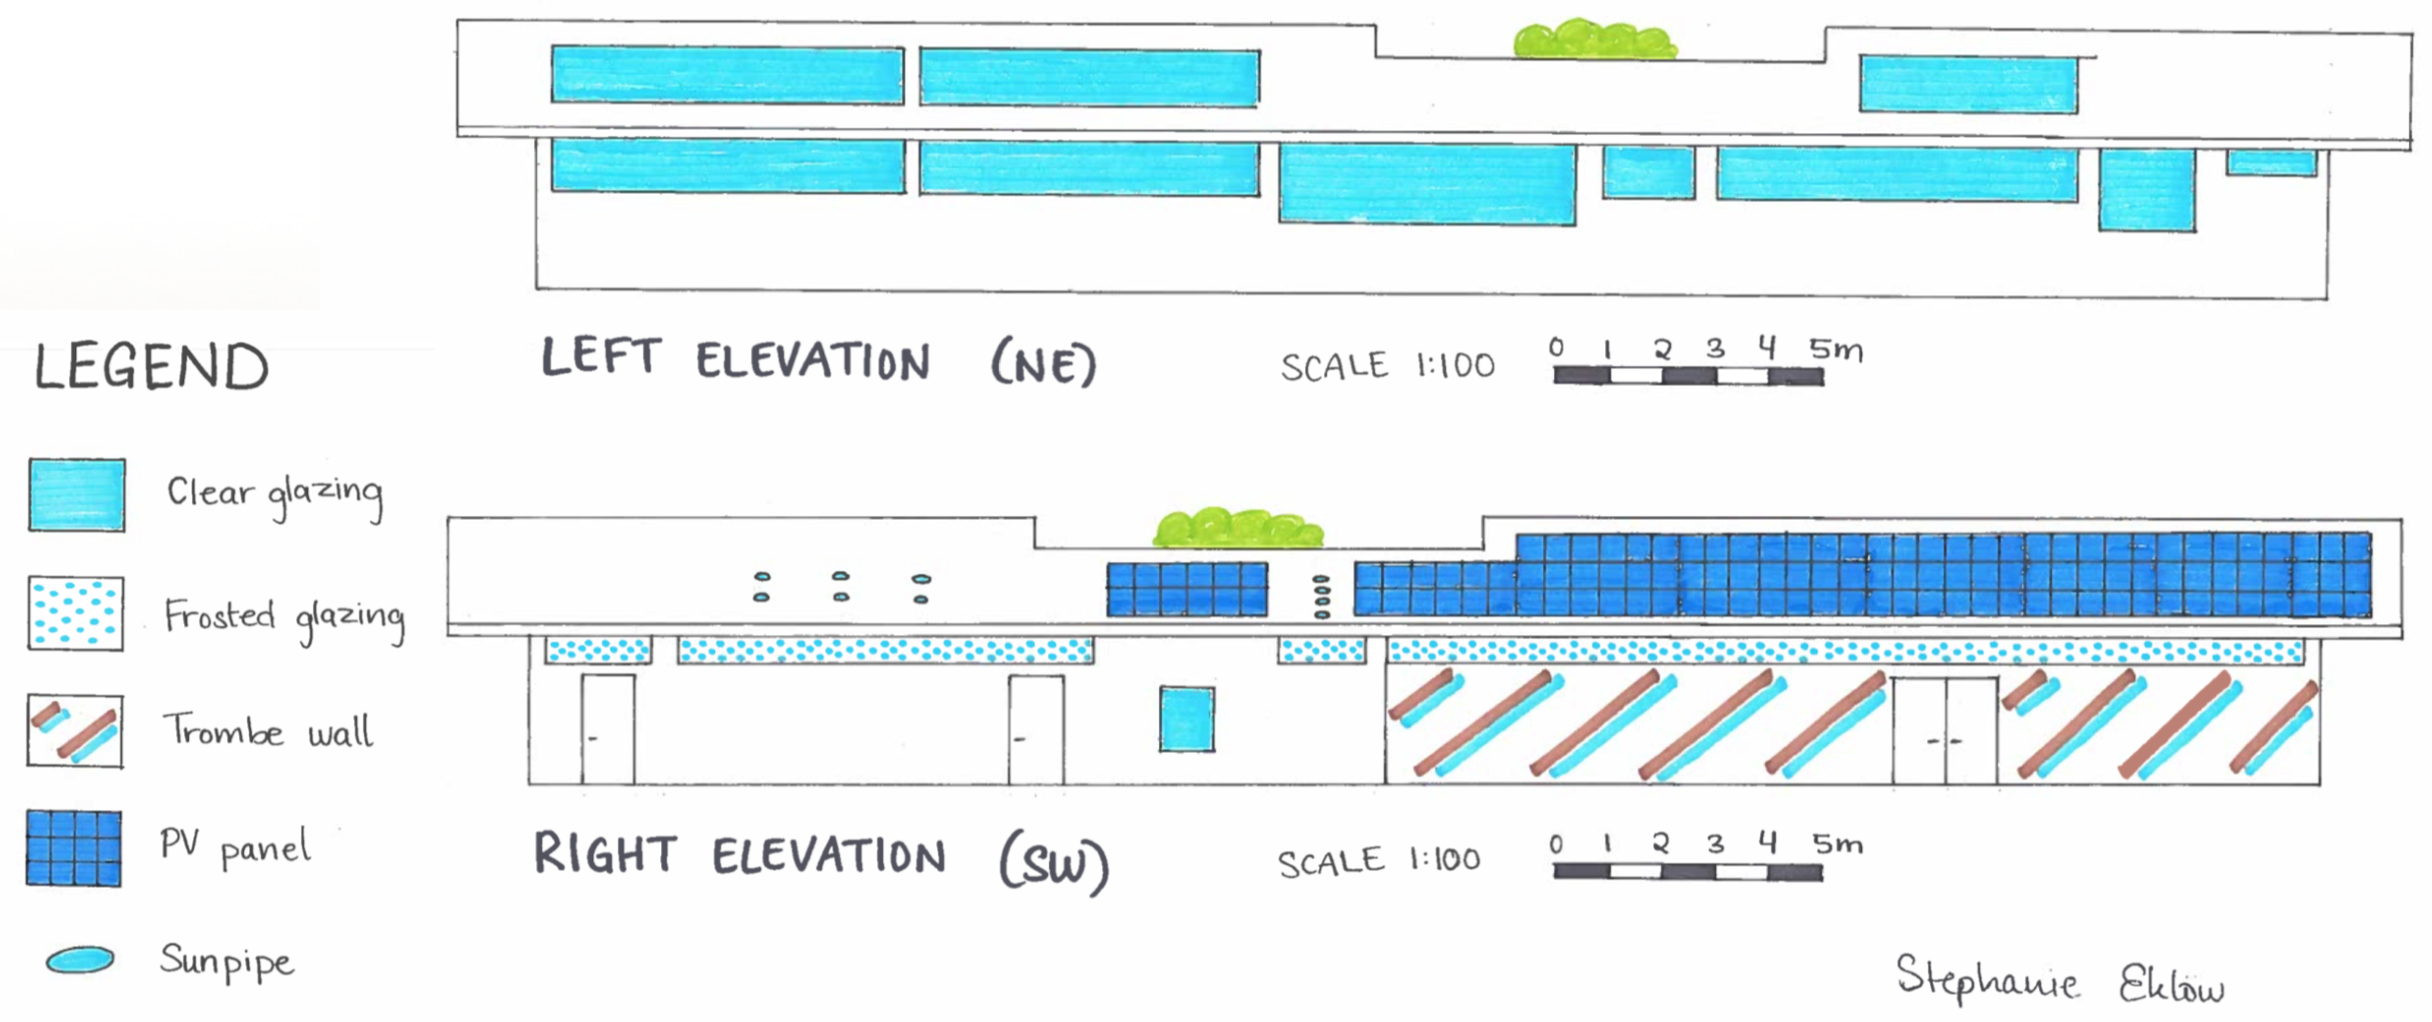
\includegraphics[width=\textwidth]{figures/NL-nl.png}
	\rule{\textwidth}{0.5pt} % use line???
	\caption{The fit-for-purpose glazing scheme of Newington Library.}
	\label{fig:nl}
\end{figure}

%\hl{If I look overll at all the steps (integrated), I can go down that path. but if I just look at the step that isn't working, I'd go down another path. Look at something that wasn't working, and . CCSA eposter: not to miss point of question/ topic (how to harness lessons from past climate events); focusing on other parts of question sets us up to fail. Because I know about this, I can apply it to engineering in the following ways. Sunamp PISs. Made sure whole process was more carefully thought out than it was when I was given the job. I had an overview of the whole thing. I made sure that the document enabled people to use the batteries as efficiently as possible. Can't do that by looking at each point of its own - it's got to flow as a document. specific application of heat batteries  - know-how  of technology and application (0.5 page)}








\newpage
\subsection*{EA5m}

\begin{wraptable}{r}{0.2\textwidth}
	\begin{tabular}{|ll|}
		\hline
		\multicolumn{2}{|c|}{\cellcolor[HTML]{F8A102}\textbf{EA5m \master}} \\ \hline
		\EnBldgs & \PRJ \\
		\DST & \ICP \\
		Hoare Lea & Sunamp \\ \hline
	\end{tabular}
\end{wraptable}

Some courses and placements have enabled me to develop my ability to use fundamental knowledge to investigate new and emerging technologies.
My most extensive investigation is of Sunamp's heat batteries, having developed the PISs and a Product Selection Quiz for their UniQ product range (see Appendices~\ref{App:PISs} and \ref{App:quiz}).
My knowledge of heat exchangers (gained notably in the thermofluids part of the \LABTitle),
water supply and heating (gained in the \PRJTitle),
and renewable technologies (gained in \EnBldgsTitle)
contributed to my understanding of the operation of Sunamp's heat batteries.










\subsection*{EA6m} \label{sec:EA6m}

\begin{wraptable}{r}{0.2\textwidth}
	\begin{tabular}{|ll|}
		\hline
		\multicolumn{2}{|c|}{\cellcolor[HTML]{F8A102}\textbf{EA6m \littlemaster}} \\ \hline
		\multicolumn{2}{|c|}{\PRJ} \\ \hline
	\end{tabular}
\end{wraptable}

I do not have a lot of experience extracting and evaluating pertinent data to apply engineering analysis techniques in the solution of unfamiliar problems.
The only example I can think of is when I tried to calculate the yield of tidal power for the \textit{4th year collaborative project}, which was part of the \PRJTitle.
This was an unfamiliar problem and I could only find information online on how to calculate yields from hydroelectric dams.
Thus, I had to use a combination of the information I found, assumptions and my own fundamental mathematical skill set.
I found that four bi-directional turbines with a total of four ebb and flood tides of three metres could generate a daily total of 284~kWh, but this was only 16\% of the building's daily electricity demand.
Since I never showed my workings to anyone, I cannot be sure if they were correct.
Overall, I believe I could use some more development in this skill area.
